\documentclass[11pt, a4paper, twoside]{article}   	% use "amsart" instead of "article" for AMSLaTeX format

\usepackage{geometry}                		% See geometry.pdf to learn the layout options. There are lots.
\usepackage{pdfpages}
\usepackage{caption}
\usepackage{minted}
\usepackage[german]{babel}			% this end the next are needed for german umlaute
\usepackage[utf8]{inputenc}
\usepackage{color}
\usepackage{graphicx}
\usepackage{titlesec}
\usepackage{fancyhdr}
\usepackage{lastpage}
\usepackage{hyperref}
\usepackage[autostyle=false, style=english]{csquotes}
\usepackage{mathtools}
\usepackage{tabularx}
% http://www.artofproblemsolving.com/wiki/index.php/LaTeX:Symbols#Operators
% =============================================
% Layout & Colors
% =============================================
\geometry{
   a4paper,
   total={210mm,297mm},
   left=20mm,
   right=20mm,
   top=20mm,
   bottom=30mm
 }	

\definecolor{myred}{rgb}{0.8,0,0}
\definecolor{mygreen}{rgb}{0,0.6,0}
\definecolor{mygray}{rgb}{0.5,0.5,0.5}
\definecolor{mymauve}{rgb}{0.58,0,0.82}

\setcounter{secnumdepth}{4}


% the default java directory structure and the main packages
\newcommand{\srcDir}{/src/main/java}
% =============================================
% Code Settings
% =============================================
\newenvironment{code}{\captionsetup{type=listing}}{}
\newmintedfile[cppSourceFile]{cpp}{
	linenos=true, 
	frame=single, 
	breaklines=true, 
	tabsize=2,
	numbersep=5pt,
	xleftmargin=10pt,
	baselinestretch=1,
	fontsize=\footnotesize
}
\newmintinline[inlineCpp]{cpp}{}
\newminted[cppSource]{cpp}{
	breaklines=true, 
	tabsize=2,
	autogobble=true,
	breakautoindent=false
}
% =============================================
% Page Style, Footers & Headers, Title
% =============================================
\title{Übung 1}
\author{Thomas Herzog}

\lhead{Übung 1}
\chead{}
\rhead{
\includegraphics[scale=0.10]{FHO_Logo_Students.jpg}}

\lfoot{S1610454013}
\cfoot{}
\rfoot{ \thepage / \pageref{LastPage} }
\renewcommand{\footrulewidth}{0.4pt}
% =============================================
% D O C U M E N T     C O N T E N T
% =============================================
% =============================================
% 2016.10.13: 1 
% 2016.10.14: 2
% =============================================

\pagestyle{fancy}
\begin{document}
\setlength{\headheight}{15mm}
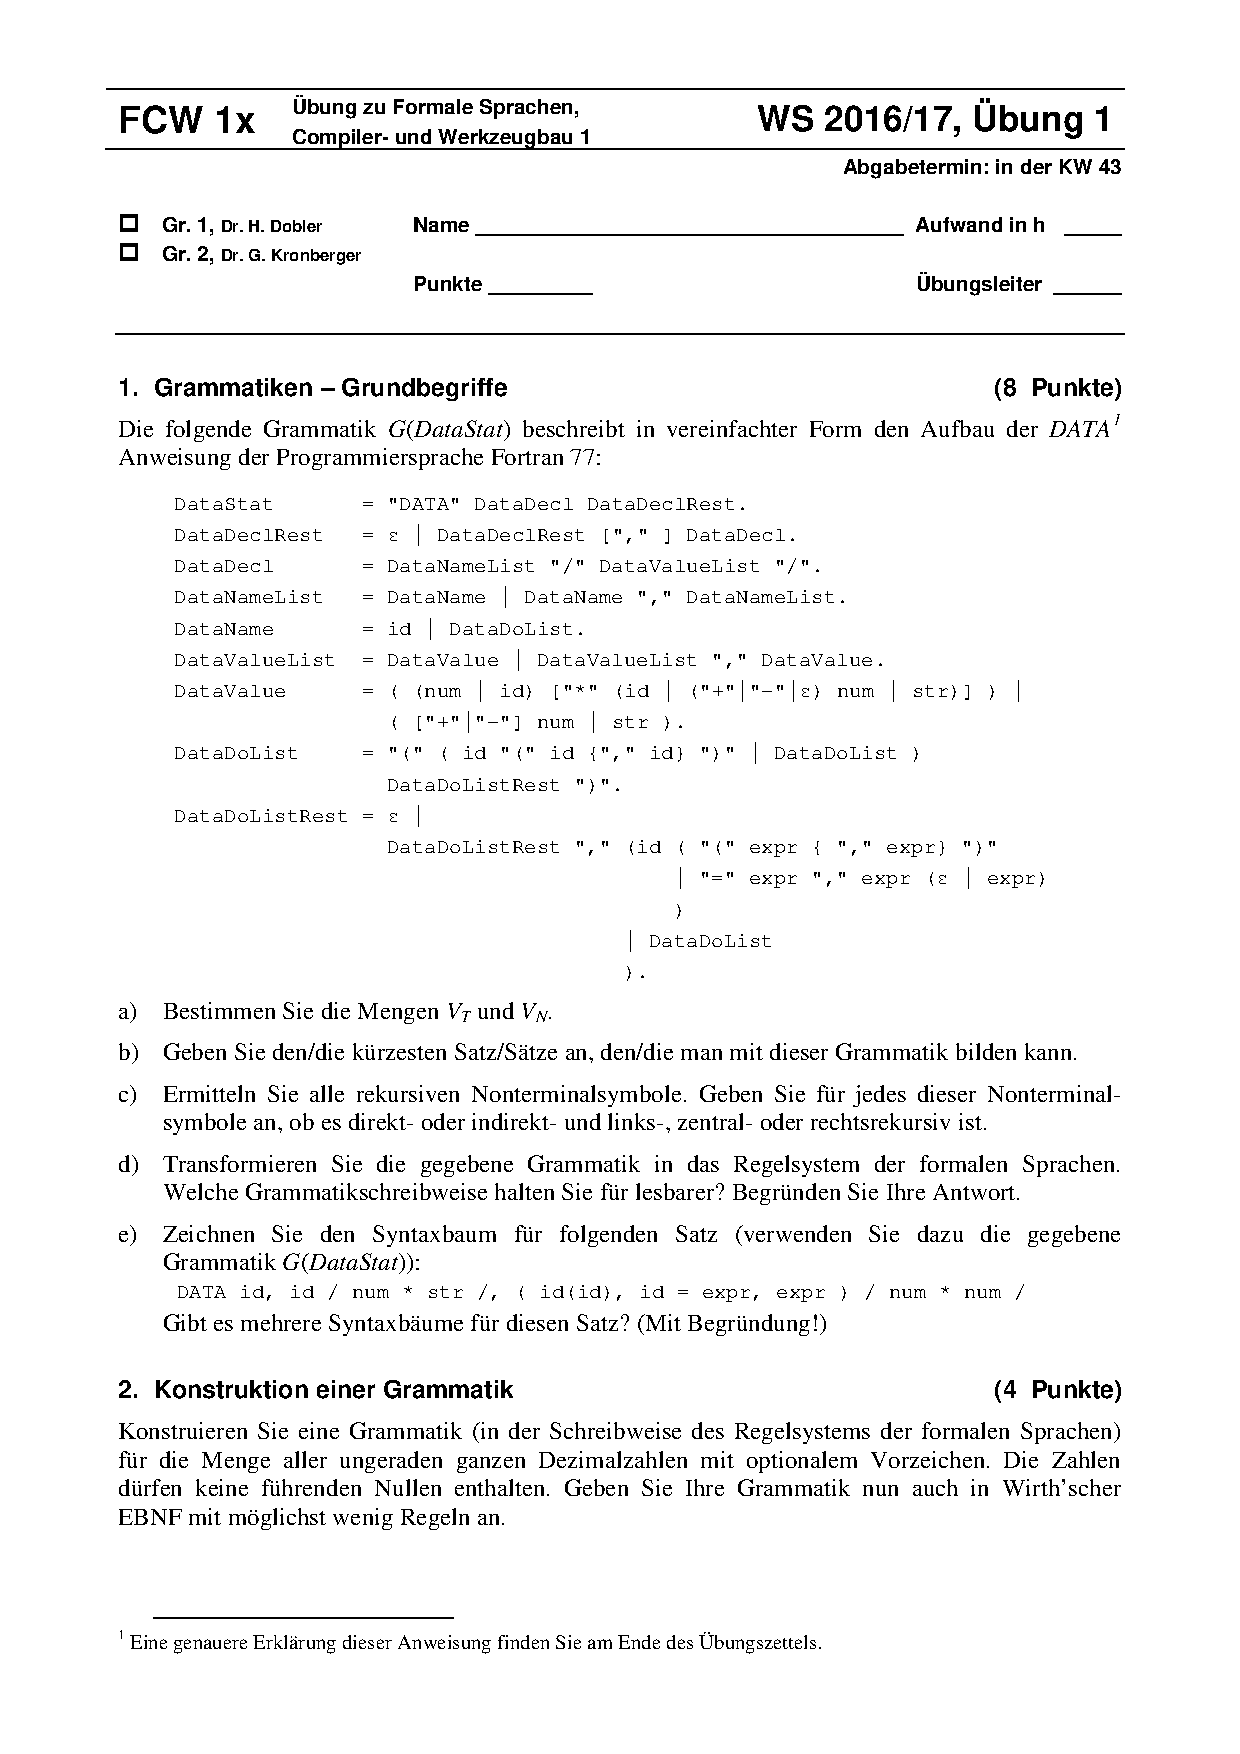
\includepdf[pages={1,2}]{Fcw1x01A.pdf}

% Section gramar and basics 
\section {Grammatiken - Grundbegriffe}
\label{sec:grammar-basics}
Dieser Teil der Dokumentation behandelt die Aufgabe 1 der ersten Übung.
\subsection{Die Mengen $V_{T}$ und $V_{N}$}
$V_{N}=\{$ DataStat, DataDeclRest, DataDecl, DataNameList, DataName, DataValueList, DataValue, DataDoList, DataDoListRest $\}$
\newline
\newline
Alle Nichtterminalsymbole befinden sich links in der Grammatik, wobei das Nichtterminalsymbol \emph{DataStat} das Satzsymbol ist.
\newline
\newline
\newline
$V_{T}=\{$ \enquote{DATA},\enquote{,}, \enquote{/}, \enquote{(}, \enquote{)},\enquote{=}, \enquote{*}, \enquote{+}, \enquote{-}, \enquote{=}, expr, id, num, str $\}$
\newline
\newline
Alle Terminalsymbole kommen nicht auf der linken Seite der Grammatik vor und können nicht weiter abgeleitet werden. Das Symbol \enquote{$\epsilon$} ist ein Metasymbol, dass die leere Kette repräsentiert und ist weder ein Nichtterminalsymbol oder ein Terminalsymbol.
\newline
\newline
\newline
$V=V_{T} \cup V_{N}$
\newline
\newline
Die Menge $V$ ist das Alphabet der Grammatik und ist die Vereinigung der Menge der Nichtterminalsymbole und der Menge der Terminalsymbole. Da das Symbol $\epsilon$ ein Metasymbol ist, ist es nicht Teil der Grammatik und auch kein Teil des Alphabets der Grammatik.

\subsection{Kürzeste Sätze der Grammatik}
DataStat $\xRightarrow{L}$ \enquote{DATA} \underline{DataDecl} DataDeclRest
\newline
\null\hspace{1.55cm} $\xRightarrow{L}$ \enquote{DATA} \underline{DataNameList} \enquote{/} DataValueList \enquote{/} DataDeclRest
\newline
\null\hspace{1.55cm} $\xRightarrow{L}$ \enquote{DATA} \underline{DataName} \enquote{/} DataValueList \enquote{/} DataDeclRest
\newline
\null\hspace{1.55cm} $\xRightarrow{L}$ \enquote{DATA} id \enquote{/} \underline{DataValueList} \enquote{/} DataDeclRest
\newline
\null\hspace{1.55cm} $\xRightarrow{L}$ \enquote{DATA} id \enquote{/} \underline{DataValue} \enquote{/} DataDeclRest
\newline
\null\hspace{1.55cm} $\xRightarrow{L}$ \enquote{DATA} id \enquote{/} num  \enquote{/} \underline{DataDeclRest}
\newline
\null\hspace{1.55cm} $\xRightarrow{L}$ \enquote{DATA} id \enquote{/} num  \enquote{/}
\newline
\newline
\newline
%
DataStat $\xRightarrow{L}$ \enquote{DATA} \underline{DataDecl} DataDeclRest
\newline
\null\hspace{1.55cm} $\xRightarrow{L}$ \enquote{DATA} \underline{DataNameList} \enquote{/} DataValueList \enquote{/} DataDeclRest
\newline
\null\hspace{1.55cm} $\xRightarrow{L}$ \enquote{DATA} \underline{DataName} \enquote{/} DataValueList \enquote{/} DataDeclRest
\newline
\null\hspace{1.55cm} $\xRightarrow{L}$ \enquote{DATA} id \enquote{/} \underline{DataValueList} \enquote{/} DataDeclRest
\newline
\null\hspace{1.55cm} $\xRightarrow{L}$ \enquote{DATA} id \enquote{/} \underline{DataValue} \enquote{/} DataDeclRest
\newline
\null\hspace{1.55cm} $\xRightarrow{L}$ \enquote{DATA} id \enquote{/} id  \enquote{/} \underline{DataDeclRest}
\newline
\null\hspace{1.55cm} $\xRightarrow{L}$ \enquote{DATA} id \enquote{/} id  \enquote{/}
\newpage

\parindent0pt DataStat $\xRightarrow{L}$ \enquote{DATA} \underline{DataDecl} DataDeclRest
\newline
\null\hspace{1.55cm} $\xRightarrow{L}$ \enquote{DATA} \underline{DataNameList} \enquote{/} DataValueList \enquote{/} DataDeclRest
\newline
\null\hspace{1.55cm} $\xRightarrow{L}$ \enquote{DATA} \underline{DataName} \enquote{/} DataValueList \enquote{/} DataDeclRest
\newline
\null\hspace{1.55cm} $\xRightarrow{L}$ \enquote{DATA} id \enquote{/} \underline{DataValueList} \enquote{/} DataDeclRest
\newline
\null\hspace{1.55cm} $\xRightarrow{L}$ \enquote{DATA} id \enquote{/} \underline{DataValue} \enquote{/} DataDeclRest
\newline
\null\hspace{1.55cm} $\xRightarrow{L}$ \enquote{DATA} id \enquote{/} str  \enquote{/} \underline{DataDeclRest}
\newline
\null\hspace{1.55cm} $\xRightarrow{L}$ \enquote{DATA} id \enquote{/} str  \enquote{/}
\newline
\newline
Das Nichtterminalsymbol \emph{DataValue} kann in drei Varianten abgeleitet werden, \emph{id}, \emph{num} und \emph{str}. Die Satzlänge bleibt bei jeder der drei Ableitungen des Nichtterminalsymbols \emph{DataValue} gleich.

\subsection{Rekursionen der Nichtterminalsymbole}
    \begin{tabularx}{\textwidth}{|>{\centering}X|>{\centering}X|>{\centering\arraybackslash}X|}
    \hline
    \textbf{Nichtterminalsymbol} & \textbf{direkt/indirekt rek.} & \textbf{links/rechts rek.} \\ \hline
    DataDeclRest                 &           direkt rek.         &           links rek.\\ \hline
    DataDecl                     &               -               &             -           
    \\ \hline
    DataNameList                 &           direkt rek.         &           rechts rek. \\ \hline
    DataName                     &               -               &             -    
    \\ \hline
    DataValueList                &           direkt rek.         &           links rek. \\ \hline
    DataValue                    &               -               &             -    
    \\ \hline
    DataDoList                   &           direkt rek.         &           zentral rek.\\ \hline
    DataDoList                   &           indirekt rek.       &           zentral rek.\\ \hline
    DataDoListRest               &           indirekt rek.       &           zentral rek.\\ \hline
    \end{tabularx}
\newline
\newline
Die beiden indirekten Rekursionen der Nichtterminalsymbole \emph{DataDoList} und \emph{DataDoListRest} ergeben sich aus der Tatsache, dass wenn es eine indirekte Rekursion gibt, es auch eine zweite Rekursion geben muss. Ich gehe davon aus, dass ich alle Rekursionen gefunden habe, wobei angemerkt sei, dass es sehr schwer ist Rekursionen aus einer Grammatik auszulesen. 

\subsection{Transformation in das Regelsystem der formalen Sprachen}
\begin{tabularx}{\textwidth}{p{80pt} @{$\rightarrow$ \hspace{10pt}} X}
	DataStat      & DATA DataDecl DataDeclRest \\
	DataDeclRest  &  $\epsilon$ $|$  DataDeclRest , DataDecl $|$ DataDeclRest   DataDecl  \\
	DataDecl       & DataNameList / DataValueList /\\
	DataNameList   & DataName $|$ DataName , DataNameList\\
	DataName       & id $|$ DataDoList\\
	DataValueList  & DataValue $|$ DataValueList , DataValue\\
	DataValue      & num DerefValue $|$ id DerefValue $|$ NumOrStr\\
	NumValue       & num $|$ + num $|$ - num\\
	NumOrStr       & NumValue $|$ str\\
	DerefValue     & $\epsilon$ $|$ * id $|$ * NumOrStr\\
	DataDoList     & ( IdList DataDoListRest ) $|$ ( DataDoList DataDoListRest )\\
	CommaId        & $\epsilon$ $|$ , id CommaId\\
    IdList         & id ( id CommaId )	\\
    DataDoListRest & $\epsilon$ $|$ DataDoListRest , DoListRestOpt \\
    ComaExpr       & $\epsilon$ $|$ , expr CommaExpr\\
    ExprList       & ( expr CommaExpr )\\
    OptExpr        & $\epsilon$ $|$ expr\\
    EqualExpr      & = expr , expr OptExpr\\
    DoListRestOpt & id ExprList $|$ id EuqlExpr $|$ DataDoList
\end{tabularx}
\newpage
Um diesen Punkt der Aufgabe \ref{sec:grammar-basics} zu lösen wurden die Optionen und Schleifen von innen nach außen aufgelöst und in eigene Nichtterminalsybole ausgelagert. Das ist notwendig, da das Regelwerk der formalen Sprachen diese Konstrukte nicht kennt und die Konstrukte Optionen und Schleifen in Oder Konstrukte umgewandelt werden müssen. Bsp.: [num, str] $\equiv$ $\epsilon$ $|$ num $|$ str
\newline
\newline
Ich halte die Schreibweise der Wirth'schen EBNF für lesbarer, da in dieser Schreibweise mehr Konstrukte wie Optionen und Schleifen zur Verfügung stehen und dadurch die Grammatik durch weniger Regeln definiert werden kann, was die Grammatik übersichtlicher macht.



%\subsubsection{MainFX.java}
%Diese Klasse stellt die Main Klasse für die JavaFX Applikation dar.
%\begin{code}
%	\caption{MainFX.java}
%	\javaSourceFile{\fxSource/main/MainFX.java}
%\end{code}
\end{document}